
\documentclass{fancyslides}

\usepackage[utf8]{inputenc} % Allows the usage of non-english characters
\usepackage{times} % Use the Times font
\usepackage{booktabs} % Allows the use of \toprule, \midrule and \bottomrule in tables
\usepackage{amsmath}
\usepackage{animate}
\graphicspath{{images/}} % Location of the slide background and figure files

% Beamer options - do not change
\usetheme{default} 
\setbeamertemplate{navigation symbols}{} % Disable the slide navigation buttons on the bottom of each slide
\setbeamercolor{structure}{fg=\yourowntexcol} % Define the color of titles and fixed text elements (e.g. bullet points)
\setbeamercolor{normal text}{fg=\yourowntexcol} % Define the color of text in the presentation

%------------------------------------------------
% COLORS
% The following colors are predefined in this class: white, black, gray, blue, green and orange

% Define your own color as follows:
%\definecolor{pink}{rgb}{156,0,151}

\newcommand{\structureopacity}{1} % Opacity (transparency) for the structure elements (boxes and circles)

\newcommand{\strcolorb}{white}
\newcommand{\strcolor}{green} % Set the color of structure elements (boxes and circles)
\newcommand{\yourowntexcol}{black} % Set the text color

%----------------------------------------------------------------------------------------
%	TITLE SLIDE
%----------------------------------------------------------------------------------------

\newcommand{\titlephrase}{\LARGE Length-SRA figs} % Presentation title
%\newcommand{\name}{Catarina Wor} % Presenter's name
%\newcommand{\affil}{UBC} % Presenter's institution
%\newcommand{\email}{catarinawor@gmail.com} % Presenter's email address
%\newcommand{\collaborators}{Co-authors: Carl Walters, Steve Martell and Murdoch McAllister}

\begin{document}


%\startingslide % This command inserts the title slide as the first slide




%------------------------------------------------

%------------------------------------------------


\begin{frame}
\begin{center} %left bottom right top,
\begin{figure}               
                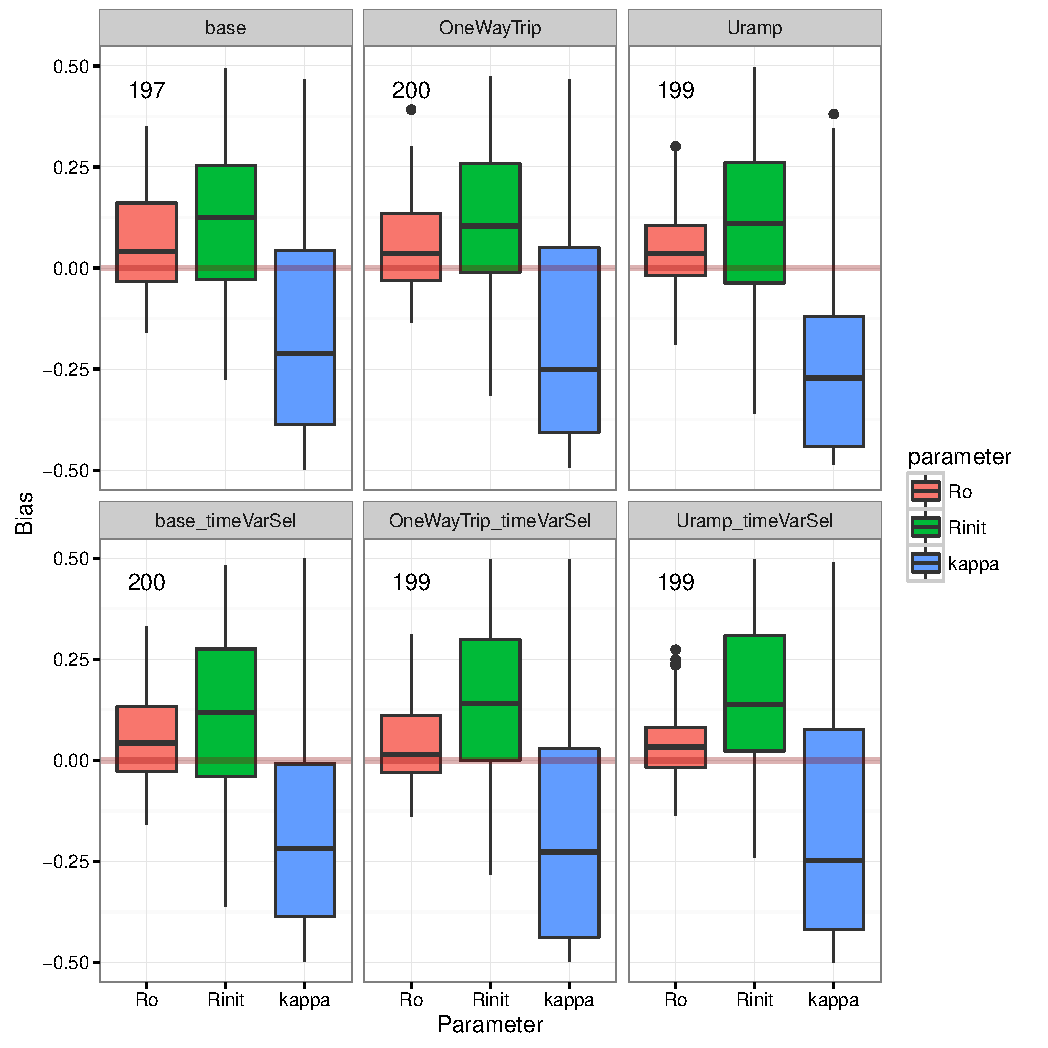
\includegraphics[trim= 0mm 0mm 0mm 0mm, scale=0.5]{main_params.pdf}  

                
\end{figure}
\end{center}
\end{frame}

%------------------------------------------------

\begin{frame}
\begin{center} %left bottom right top,
\begin{figure}               
                \includegraphics[trim= 0mm 0mm 0mm 0mm, scale=0.5]{derivQuant.pdf}  
\end{figure}
\end{center}
\end{frame}

%------------------------------------------------


\begin{frame}
\begin{center} %left bottom right top,
\begin{figure}               
                \includegraphics[trim= 0mm 0mm 0mm 0mm, scale=0.5]{U_bias.pdf}  
\end{figure}
\end{center}
\end{frame}

%------------------------------------------------


%------------------------------------------------


\begin{frame}
\begin{center} %left bottom right top,
\begin{figure}               
                \includegraphics[trim= 0mm 0mm 0mm 0mm, scale=0.5]{Sbiomass.pdf}  
\end{figure}
\end{center}
\end{frame}

%------------------------------------------------

%------------------------------------------------


\begin{frame}
\begin{center} %left bottom right top,
\begin{figure}               
                \includegraphics[trim= 0mm 0mm 0mm 0mm, scale=0.5]{RecDev_bias.pdf}  
\end{figure}
\end{center}
\end{frame}

%------------------------------------------------

%------------------------------------------------


\begin{frame}
\begin{center} %left bottom right top,
\begin{figure}               
                \includegraphics[trim= 0mm 0mm 0mm 0mm, scale=0.5]{UlengthMedian.pdf}  
\end{figure}
\end{center}
\end{frame}


%------------------------------------------------



\end{document}